\documentclass[12pt]{article}
\title{ECE 141 Homework 2}
\usepackage{subcaption}
\author{Lawrence Liu}
\usepackage{graphicx}
\usepackage{amsmath}
\usepackage{placeins}
\newcommand{\Laplace}{\mathscr{L}}
\setlength{\parskip}{\baselineskip}%
\setlength{\parindent}{0pt}%
\usepackage{xcolor}
\usepackage{listings}
\definecolor{backcolour}{rgb}{0.95,0.95,0.92}
\usepackage{amssymb}
\lstdefinestyle{mystyle}{
    backgroundcolor=\color{backcolour}}
\lstset{style=mystyle}

\begin{document}
\maketitle
\section*{Problem 6.5}

This has two break points, one at $\omega=1$ and another at $\omega=2$. Furthermore because of the $\frac{1}{s}$, we
have that the sketch of the bode plots look like.\\
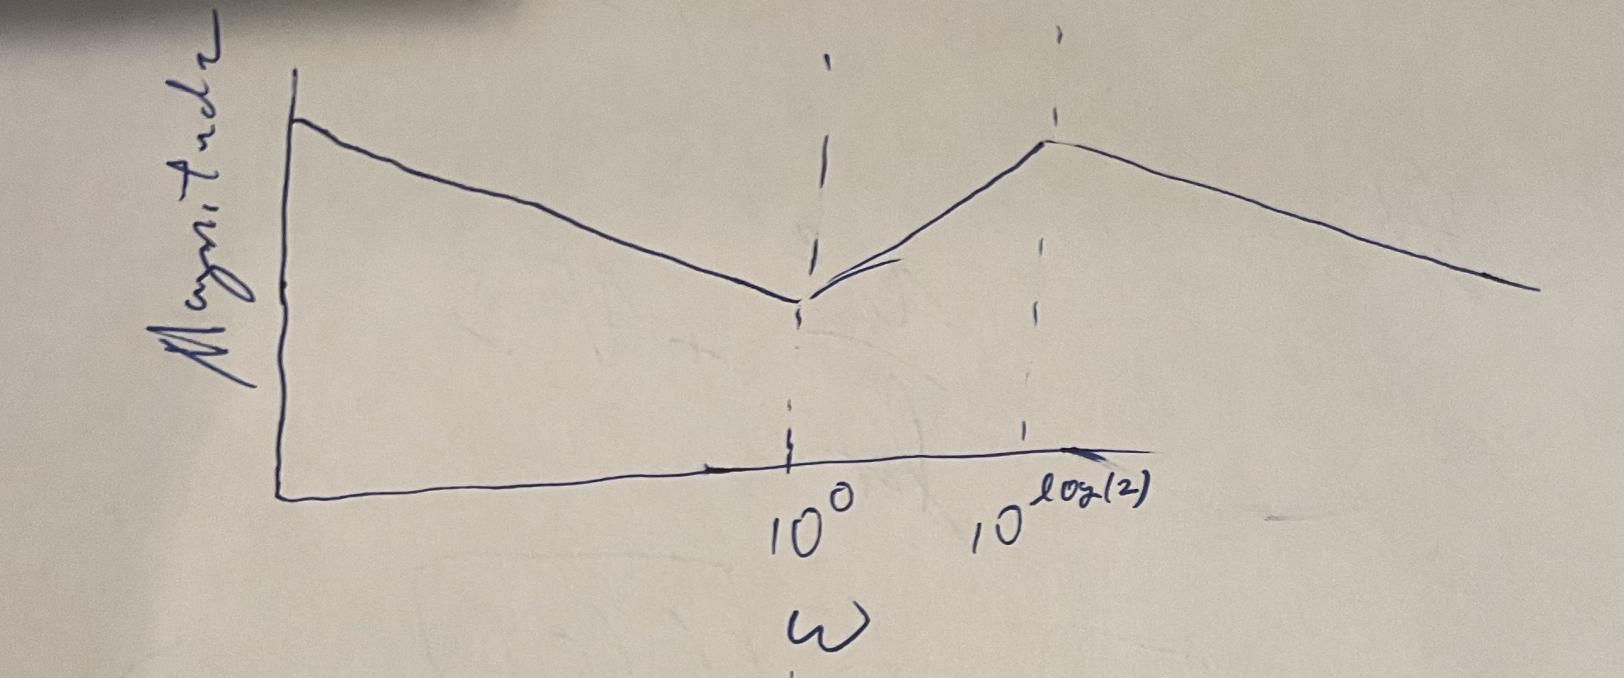
\includegraphics[scale=0.2]{Problem1Fig1.png}\\
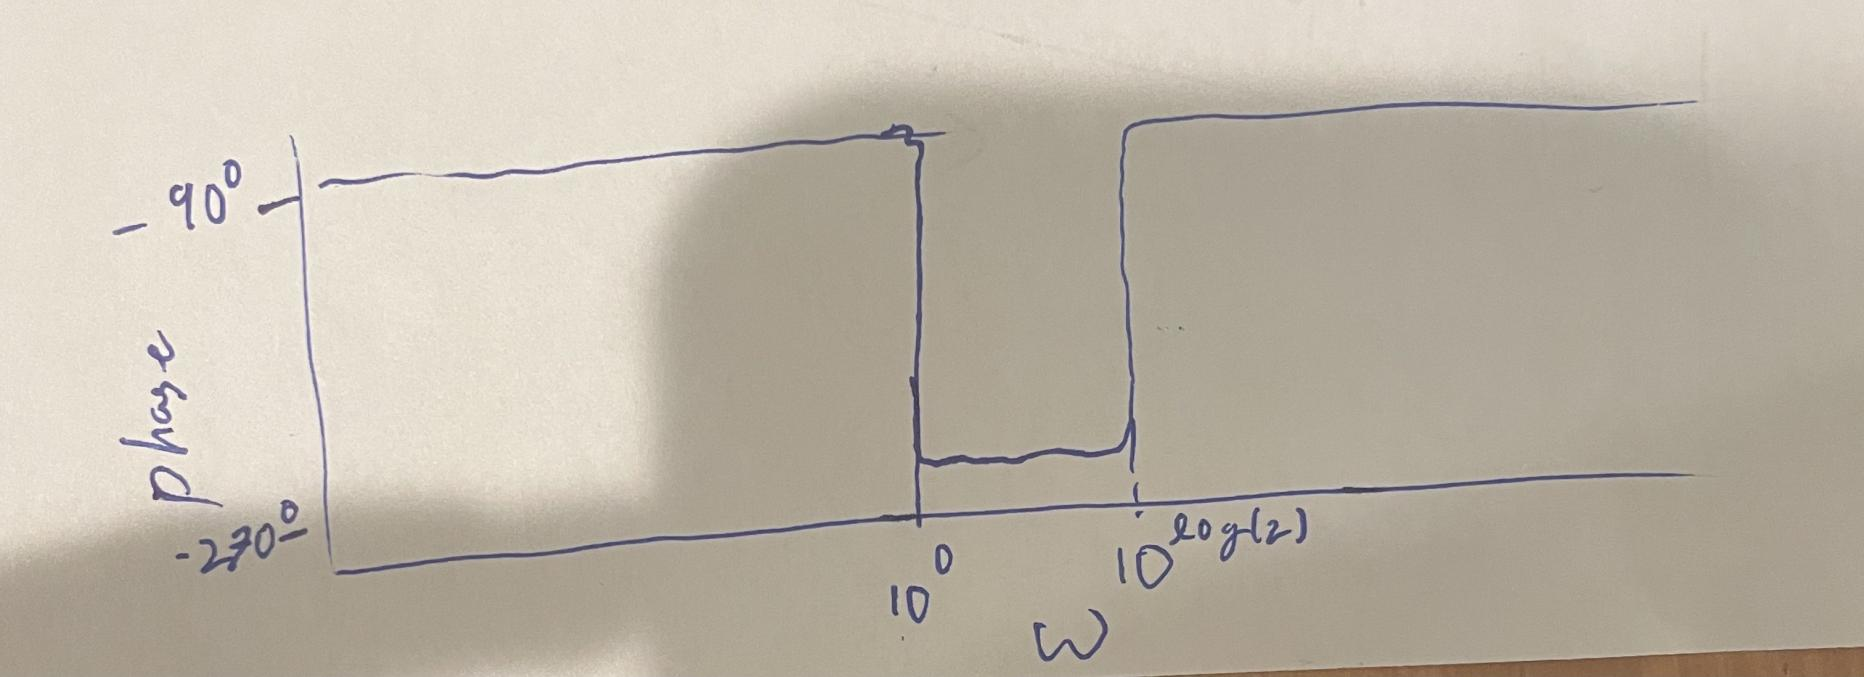
\includegraphics[scale=0.2]{Problem1Fig2.jpg}\\
We can confirm this with the following matlab code
\begin{verbatim}
sys = tf([1 0 4], [1 0 1 0]);
bode(sys)
\end{verbatim}
Which outputs the following plot\\
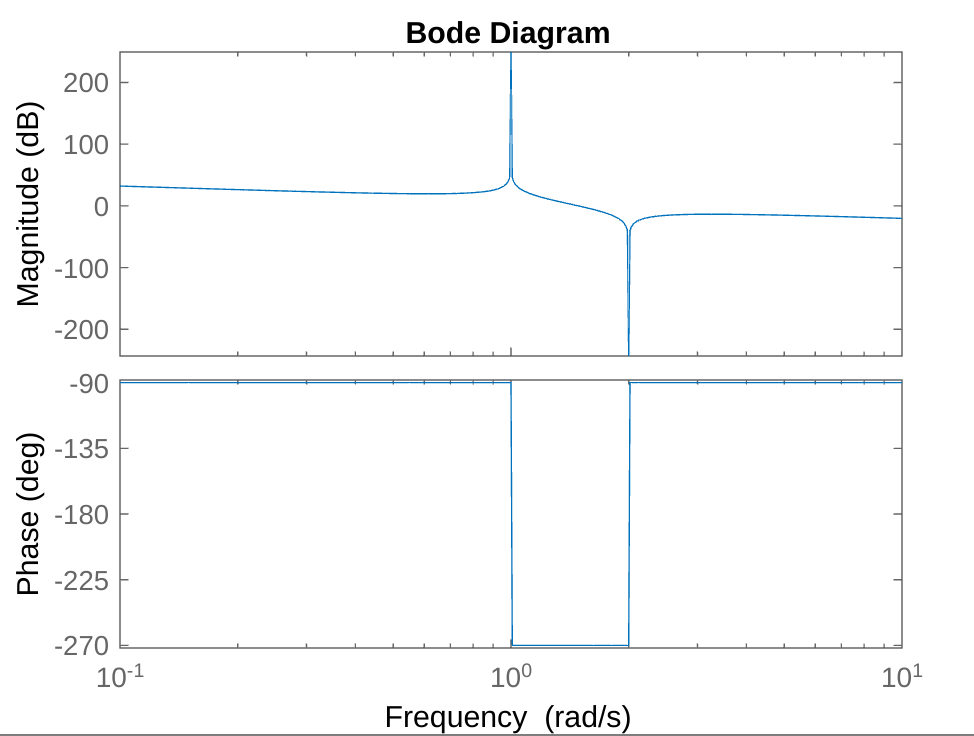
\includegraphics[scale=0.2]{Problem1Fig3.png}\\
\section*{Problem 6.7}

\end{document}